\newcommand{\content}{
    

    

    % добавляем нумерацию
    \AddToShipoutPicture{
        \begin{textblock*}{1cm}(19.5cm,28.6cm) % Ширина блока, координаты (x, y)
                \centering 
                \number\numexpr\thepage+1\relax
        \end{textblock*}
    }

    % добавляем шифр
    \AddToShipoutPicture{
        \begin{textblock*}{10cm}(9cm,28.2cm) % Ширина блока, координаты (x, y)
            \centering
            \chipher
        \end{textblock*}
    }

    % шифр на 1ый лист
    \begin{textblock*}{10cm}(9cm,28.2cm) % Ширина блока, координаты (x, y)
        \centering
        \chipher
    \end{textblock*}

    \section{\MakeUppercase{Введение}}
    {
        В современном мире стремительного развития технологий обработки и анализа данных задача автоматической классификации текстовых данных, включая языки программирования, становится особенно актуальной. Она открывает новые возможности для обучения нейронных сетей, повышения безопасности информационных систем и улучшения пользовательского опыта в мессенджерах.

        Классификация программного кода играет ключевую роль в создании структурированных данных для обучения крупных языковых моделей. Эти модели, такие как трансформеры, требуют чистых и четко классифицированных данных, чтобы эффективно различать текст на разных языках и работать со смешанными типами информации. Применение методов классификации позволяет не только улучшить качество таких моделей, но и значительно ускорить подготовку данных.
        
        Кроме того, растет значение анализа кода, передаваемого через текстовые сообщения в мессенджерах, таких как Telegram. Увеличение объема такого рода информации создает как новые возможности для сотрудничества разработчиков, так и риски, связанные с вредоносными скриптами и фишингом. Автоматическая классификация помогает защитить пользователей, идентифицируя и блокируя потенциально опасный контент.
        
        Разработка технологий, способных отличать программный код от обычного текста, также важна для повышения уровня кибербезопасности. Такие системы могут применяться для фильтрации вредоносных сообщений, предотвращения атак с использованием кода и защиты информационных систем.
        
        Таким образом, создание методов классификации языков программирования с использованием сверточных нейронных сетей не только повышает эффективность анализа данных, но и способствует решению задач безопасности и оптимизации процессов в сфере информационных технологий.
    }
    \newpage

\newpage
\section{\MakeUppercase{Постановка задачи}}

Целью данной работы является разработка системы классификации текстовых данных с целью определения языка программирования, основанной на методах глубокого обучения. В качестве базовой модели будет использоваться предварительно обученная сверточная нейронная сеть, которая будет дообучаться (файнтюниться) на специализированном датасете, содержащем фрагменты кода на различных языках программирования.

Задачи, которые необходимо решить в рамках проекта:
\begin{enumerate}
    \item \textbf{подготовка набора данных;} \\
    Необходимо собрать и подготовить набор текстов, содержащих примеры программного кода на различных языках, а также отфильтровать их от нерелевантной информации. Важно учесть разнообразие языков программирования, а также сбалансированность данных по количеству примеров для каждого языка. Также требуется подготовить текстовые данные для последующего подачи в модель. 
    \item \textbf{выбор архитектуры базовой модели;} \\
    Проанализировать сущесвтвующие модели свертночных нейронных сетей для классификации изображений и выбрать подходящую для данной работы.
    \item \textbf{обучение (файнтюнинг) предобученной модели;} \\
    Дообучить предобученную модель на подготовленных данных с примерами программного кода. Это позволит использовать уже усвоенные моделью особенности обработки изображений и адаптировать её к специфике классификации языков программирования.
    \item \textbf{оценка качества работы модели;} \\
    После обучения модели необходимо провести её тестирование на независимом наборе данных используя метрики, такие как accuracy, F1-score, precision и recall. 
\end{enumerate}

\newpage
\section{\MakeUppercase{Выбор и описание используемых инструментов}}
{
    Для решения задачи классификации языков программирования с использованием нейронных сетей были выбраны следующие инструменты и библиотеки: 
    \begin{itemize}
        \item \textbf{requests:} это библиотека для работы с HTTP-запросами, которая позволяет удобно скачивать данные с веб-ресурсов. Она является полезной для сбора данных из открытых источников, таких как GitHub, где можно найти репозитории с примерами кода на различных языках программирования. Requests предоставляет простой и интуитивно понятный интерфейс для работы с HTTP-API, что делает процесс извлечения данных быстрым и эффективным;
        \item \textbf{Pillow:} библиотека для обработки изображений, которая позволяет работать с графическими файлами в Python. Она полезна для преобразования текстовых данных в изображения, что является важным этапом при использовании сверточных нейронных сетей, которые эффективно работают с визуальной информацией. Pillow поддерживает множество форматов изображений и предоставляет богатый функционал для обработки, что делает её удобным инструментом для работы с изображениями;
        \item \textbf{PyTorch:} один из самых популярных фреймворков для разработки и обучения нейронных сетей. PyTorch предоставляет широкие возможности для работы с различными типами архитектур, включая сверточные нейронные сети, и поддерживает эффективное использование GPU. Его гибкость и высокопроизводительные вычисления делают его идеальным инструментом для разработки сложных моделей, включая те, которые требуют тонкой настройки и оптимизации;
        \item \textbf{Kaggle:} платформа для работы с данными и машинным обучением. Kaggle предоставляет удобные средства для хранения и совместного использования датасетов, а также для обучения и тестирования моделей. Платформа поддерживает работу с вычислительными мощностями в облаке, что позволяет эффективно обучать модели на больших объемах данных без необходимости иметь собственные ресурсы. Kaggle также предоставляет инструменты для сохранения результатов и обмена ими с сообществом;
    \end{itemize}
    Эти инструменты обеспечивают гибкость, эффективность и производительность на различных этапах работы с данными и моделями, что делает их оптимальным выбором для решения задачи классификации языков программирования. 
}

\newpage
\section{\MakeUppercase{Обучение нейронной сети}}
В данном разделе описаны этапы обучения модели для классификации текстов программного кода с использованием сверточных нейронный сетей, а также процесс подготовки данных.
{
\subsection{Подготовка данных}
Подготовка данных — один из ключевых этапов в процессе обучения нейронной сети. Для эффективной классификации языков программирования, на основе данных, собранных с GitHub, были выполнены следующие шаги:
\begin{itemize}
    \item \textbf{скачивание данных:} для сбора данных использовалась библиотека re-quests, с помощью которой были скачаны файлы с кодом на 28 языках программирования, включая такие популярные языки, как Python, Java, C++, JavaScript и другие. Эти языки были выбраны на основе их распространенности и представительности в различных областях программирования. В дополнение к этому, был создан специальный класс для языков, не вошедших в основной список, а также для текстовых данных, не относящихся к программированию;
    \item \textbf{объединение данных в файлы:} каждый язык программирования был помещен в отдельный файл, который содержал код на соответствующем языке. Все файлы были объединены в один большой файл для каждого класса языкпрограммированияилитекст. Это объединение помогло организовать данные и упростить дальнейшую обработку;   
    \item \textbf{разделение данных:} для подготовки данных к обучению, все файлы были случайным образом разделены на фрагменты длиной от 64 до 1024 символов. Это важно для того, чтобы модель могла обрабатывать тексты разной длины, а также для увеличения разнообразия входных данных. В случаях, когда файл содержал меньше 1024 символов, его содержимое было дополнено путем дублирования, чтобы добиться нужной длины и обеспечить постоянство входных данных для нейронной сети;    
    \item \textbf{преобразование в изображения :} следующим шагом была обработка данных с использованием библиотеки Pillow. Каждый файл, представляющий код на определенном языке программирования или текст, был преобразован в изображение. Это преобразование позволило представить текстовую информацию в визуальной форме, что является необходимым для работы сверточных нейронных сетей.    
\end{itemize}
}

\subsection{Выбор архитектуры нейронной сети}
Для задачи классификации языков программирования, представленных в виде изображений, была выбрана модель \textbf{EfficientNetV2-S}, оригинальная архитектура которой представлена в таблице 4.1. Это небольшая версия модели \textbf{EfficientNetV2}, которая предобучена на датасете ImageNet-21k и затем дополнительно дообучалась на ImageNet-1k для задач классификации изображений. Данная модель показывает хороший баланс между временем обработки данных и
достигаемой точностью. Выбор данной модели обусловлен ее небольшим размером, неплохими результатами классификации по сравнению с другими моделями в State of Art, а также использованием механизмов внимания, что может положитьно сказаться на классификации языков, где важны мелкие детали.
Для доообучения последний слой модели был заменен на полносвязный слой, соответствующий количеству классов в задаче классификации языков программирования. Этот подход позволяет адаптировать предобученную архитектуру EfficientNetV2-S под специфику новой задачи, сохранив преимущества предварительного обучения на обширных датасетах упомянутых выше.
\begin{table}[h]
    \centering
    \renewcommand{\arraystretch}{1.5} % Увеличение вертикальных отступов
    \begin{tabular}{|p{2.5cm}|p{4cm}|p{3cm}|p{2.5cm}|} % Расширение ширины колонок
        \hline
        \textbf{Этап} & \textbf{Оператор} & \textbf{Каналы} & \textbf{Слои} \\ % Заголовки колонок
        \hline
        0 & Conv3x3 & 24 & 1 \\ 
        \hline
        1 & Fused-MBConv1, k3x3 & 24 & 2 \\ 
        \hline
        2 & Fused-MBConv4, k3x3 & 48 & 4 \\ 
        \hline
        3 & Fused-MBConv4, k3x3 & 64 & 4 \\ 
        \hline
        4 & MBConv4, k3x3, SE0.25 & 128 & 6 \\ 
        \hline
        5 & MBConv6, k3x3, SE0.25 & 160 & 9 \\ 
        \hline
        6 & MBConv6, k3x3, SE0.25 & 256 & 15 \\ 
        \hline
        7 & Conv1x1 \& Pooling \& FC & 1280 & 1 \\ 
        \hline
    \end{tabular}
    \caption{Архитектура EfficientNetV2-S}
    \label{tab:example}
\end{table}


Как видно из таблицы 4.1, основными блоками в архитектуре Efficient-NetV2-S я вляются \textbf{Fused-MBConv} и \textbf{MBConv}.

Fused-MBConv представляет собой упрощённый мобильный блок свёртки, который объединяет две операции (Depthwise и Pointwise свёртки) в одну стандартную свёртку. Это позволяет уменьшить количество вычислений и увеличить производительность, что особенно важно для задач, выполняемых на устройствах с ограниченными ресурсами. Блок состоит из двух основных этапов. Сначала применяется свёртка 3x3 с нормализацией BatchNorm и активацией SiLU, которая извлекает пространственные признаки. Затем используется свёртка 1x1 с нормализацией BatchNorm, предназначенная для уменьшения размерности каналов и снижения вычислительной сложности.

В отличие от Fused-MBConv, блок MBConv реализует более сложный подход, включающий последовательное применение Pointwise и Depthwise свёрток. Сначала происходит расширение каналов с помощью свёртки 1x1, что позволяет извлекать сложные признаки из входных данных. Далее используется Depthwise свёртка 3x3, которая обрабатывает каждый канал независимо, значительно сокращая количество параметров при сохранении пространственной информации. После этого в работу включается блок Squeeze-and-Excitation (SE), который усиливает наиболее важные признаки, выделяя значимые каналы с помощью глобального контекста. Это достигается через адаптивное усреднение, два полносвязных слоя и активацию Sigmoid. Завершающим этапом является свёртка 1x1 с нормализацией BatchNorm, возвращающая количество каналов к исходной размерности.


Как было уже сказано выше, в качестве функции активации была выбрана \textbf{SiLU} (Sigmoid Linear Unit), которая вычисляется как произведение входного значения и сигмоида от этого значения:  

\[
\text{SiLU}(x) = x \cdot \text{sigmoid}(x) = x \cdot \frac{1}{1 + e^{-x}}
\]

Главное преимущество SiLU заключается в том, что она сочетает свойства ReLU и сигмоида, обеспечивая нелинейность, необходимую для обучения сложных моделей, при этом избегая резких обнулений градиентов, характерных для ReLU. SiLU помогает модели лучше обучаться, так как она сохраняет больше информации даже для отрицательных значений входов, что снижает вероятность возникновения проблемы "мертвых" нейронов, характерной для ReLU. 

\subsection{Обучение нейронной сети}

Для обучения нейронной сети была использована функция потерь Cross-EntropyLoss, которая хорошо подходит для задач многоклассовой классификации:
\[
H(y, \hat{y}) = -\sum_{i=1} y_{i} \log(\hat{y}_{i}),
\] 
где:
\begin{itemize}
    \item H: функция потерь (кросс-энтропия), измеряющая расхождение между истинным распределением меток и прогнозируемыми вероятностями;
    \item \textbf{\(y_i\):} истинное значение для класса \(i\), которое принимает значение 1, если данный класс является правильным, и 0 в противном случае (в случае one-hot encoding меток);
    \item \textbf{\(\hat{y}_i\):} прогнозируемая вероятность принадлежности к классу \(i\) (выход модели после применения softmax).
\end{itemize}

В качестве оптимизатора применялся SGD (Stochastic Gradient Descent), обеспечивающий стабильное обучение за счёт использования метода стохастического градиентного спуска. Для повышения эффективности оптимизации использовался моментум со значением 0.9, а скорость обучения была установлена на уровне 0.001.

Выбор данных параметров позволил достичь сбалансированной производительности модели и обеспечить её стабильную сходимость в процессе обучения. На рисунке 4.1 представлен график изменения точности нейронной сети на обучающей и валидационной выборках, иллюстрирующий динамику улучшения качества модели в ходе её тренировки.
\begin{figure}[H]
    \centering
    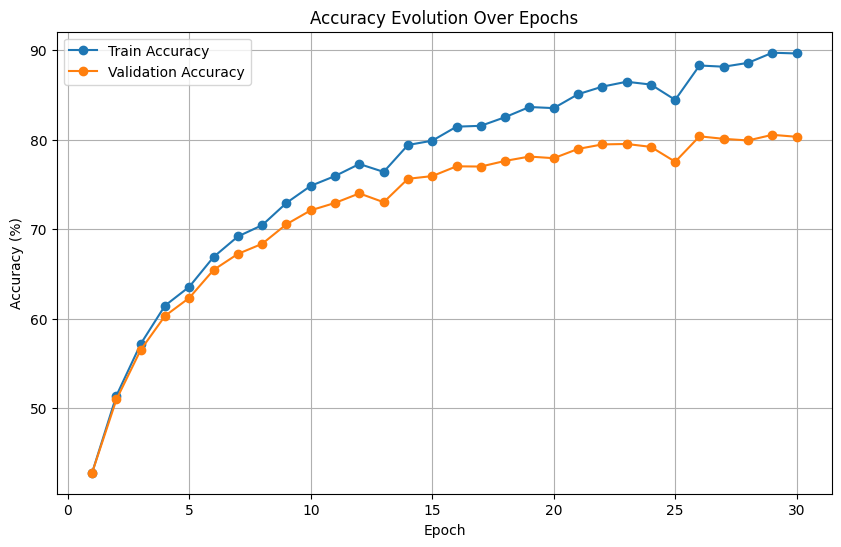
\includegraphics[width=1\textwidth]{assets/accuracy_evolution.png} 
    \caption{График ошибки при обучении}
\end{figure}

\newpage
\section{\MakeUppercase{Тестирование нейронной сети}}

В данном разделе описаны этапы тестирования обученной нейронной сети для классификации текстов программного кода. Основной целью тестирования является проверка корректности работы модели, её точности и эффективности. Тестирование включало следующие этапы:

\begin{itemize}
    \item \textbf{функциональное тестирование:} проверка работы модели на тестовых данных для анализа её способности различать положительный и отрицательный классы;
    \item \textbf{оценка качества модели:} после обучения модель тестируется на тестовой выборке. Оценка качества производится с использованием следующих метрик, представленных в таблице 5.1 и построение матрицы ошибок (нормализованной в целях упрощения визуального анализа и повышения интерпретируемости), представленной на рисунке 5.1:
    \begin{itemize}
        \item \textbf{Accuracy (точность):} процент правильных предсказаний среди всех;
        \item \textbf{F-мера:} среднее гармоническое между precision и recall;
        \item \textbf{Recall (полнота):} доля правильных положительных предсказаний;
        \item \textbf{Precision (точность):} доля правильных положительных предсказаний среди всех предсказанных положительных.
    \end{itemize}
    \item \textbf{тестирование производительности:} проверка времени выполнения модели на тестовом наборе данных, а также анализ её эффективности при обработке больших объёмов текстовой информации.
\end{itemize}
\begin{table}[h]
    \centering
    \renewcommand{\arraystretch}{1.5} % Увеличивает вертикальные отступы
    \begin{tabular}{|p{3cm}|p{3cm}|} % Увеличивает ширину колонок
        \hline
        \textbf{Метрика} & \textbf{Значение} \\ % Добавлено для улучшения читаемости
        \hline
        Precision & 0.8071 \\ 
        \hline
        Recall & 0.8054  \\ 
        \hline
        F1 Score & 0.8052  \\ 
        \hline
        Accuracy & 0.8054  \\ 
        \hline
    \end{tabular}
    \caption{Точность нейронной сети на тестовом наборе}
    \label{tab:example}
\end{table}

\begin{figure}[H]
    \centering
    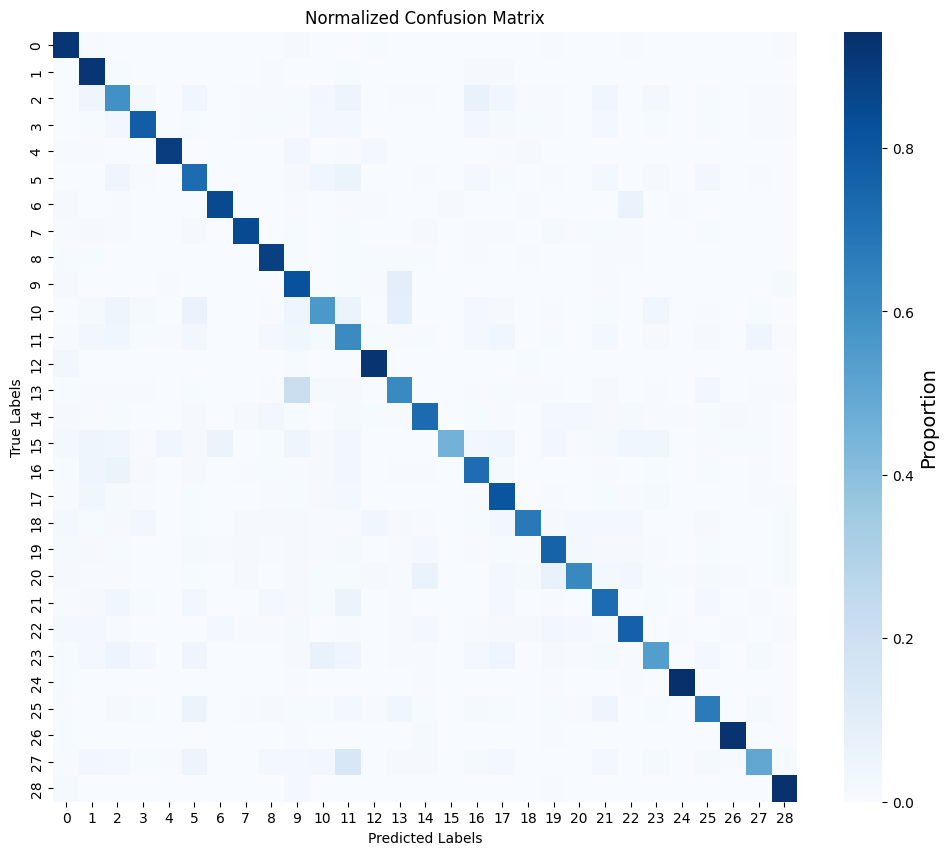
\includegraphics[width=1\textwidth]{assets/confusion.png} 
    \caption{Матрица ошибок}
\end{figure}

В результате тестирования модель показала хорошую общую точность, особенно при классификации популярных языков программирования. Основные ошибки были связаны с трудно различимыми языками и текстами, не относящимися к программированию. Для повышения точности в таких случаях планируется дополнительно расширить и улучшить данные.
\newpage
\section{\MakeUppercase{Заключение}}
В ходе выполнения курсового проекта была достигнута основная цель — разработана система классификации языков программирования с использованием сверточных нейронных сетей. Основное внимание было уделено подготовке специализированного датасета, обучению и тестированию модели на базе архитектуры EfficientNetV2-S. 

В процессе работы была реализована модель, которая эффективно классифицирует фрагменты программного кода по языкам программирования. Обучение проводилось на подготовленных данных с использованием метрик точности, F1-score, precision и recall, что позволило всесторонне оценить её эффективность. Проведённая тонкая настройка гиперпараметров и архитектуры модели позволила достичь высокой точности классификации - порядка 80\% на тестовой выборке. 

Использованные методы и технологии продемонстрировали потенциал сверточных нейронных сетей для решения задач классификации текстовых данных. Разработанная система может быть применена для автоматизации анализа программного кода, повышения безопасности информационных систем и оптимизации процессов обработки данных. 

Результаты работы показывают перспективность применения машинного обучения для классификации языков программирования. Данный проект открывает новые возможности для развития технологий анализа кода, защиты от вредоносных скриптов и улучшения взаимодействия разработчиков в информационной среде. 
\newpage
\section{Список использованной литературы}
\sloppy
{
    \begin{enumerate}
        \item Tan M., Le Q.V. EfficientNetV2: Smaller Models and Faster Training Электронныйресурс  [Электронный ресурс]. – Режим доступа: \url{https://arxiv.org/abs/2104.00298} . – Дата доступа: 19.11.2024. 
        \item Sandler M., et al. MobileNetV2: Inverted Residuals and Linear Bottlenecks [Электронный ресурс]. – Режим доступа: \url{https://arxiv.org/abs/1801.04381}. – Дата доступа: 19.11.2024.
        \item Большое сравнение 400 нейронных сетей для задачи классификации [Электронный ресурс]. – Режим доступа: \url{https://habr.com/ru/articles/666314/}. – Дата доступа: 19.11.2024.
        \item PyTorch Documentation [Электронный ресурс]. – Режим доступа: \url{https://pytorch.org/docs/stable/index.html}. – Дата доступа: 17.11.2024.
        \item Kaggle Documentation [Электронный ресурс]. – Режим доступа: \url{https://www.kaggle.com/docs}. – Дата доступа: 19.11.2024.
    \end{enumerate}
}
}